% Copyright 2004 by Till Tantau <tantau@users.sourceforge.net>.
%
% In principle, this file can be redistributed and/or modified under
% the terms of the GNU Public License, version 2.
%
% However, this file is supposed to be a template to be modified
% for your own needs. For this reason, if you use this file as a
% template and not specifically distribute it as part of a another
% package/program, I grant the extra permission to freely copy and
% modify this file as you see fit and even to delete this copyright
% notice. 

\documentclass{beamer}
\usepackage{svg}
\usepackage{hyperref}
\usepackage{tikz}
\usepackage{mathtools}
\usepackage{wrapfig}
\usepackage{amsmath}
\usepackage{adjustbox}
\usepackage{graphicx}
\usepackage[T2A]{fontenc}
\usepackage[utf8]{inputenc}
\usepackage{booktabs,tabularx}
\usepackage{makecell}
\usepackage{minted}
\usepackage[utf8]{inputenc}
\usepackage[english,russian]{babel}
 
\usepackage{minted}
    \hypersetup{colorlinks=true,linkcolor = blue,
            allbordercolors={0 0 0},
            pdfborderstyle={/S/U/W 1}}

\renewcommand{\theFancyVerbLine}{
  \sffamily\textcolor[rgb]{0.5,0.5,0.5}{\scriptsize\arabic{FancyVerbLine}}}
\renewcommand\theadalign{bc}
\renewcommand\theadfont{\bfseries}
\renewcommand\theadgape{\Gape[4pt]}
\renewcommand\cellgape{\Gape[4pt]}
\newcommand{\mybluehref}[2]{\hyperref[#1]{\color{green}\setulcolor{red}\ul{#2}}}

% \usepackage[russian]{babel}

% There are many different themes available for Beamer. A comprehensive
% list with examples is given here:
% http://deic.uab.es/~iblanes/beamer_gallery/index_by_theme.html
% You can uncomment the themes below if you would like to use a different
% one:
%\usetheme{AnnArbor}
%\usetheme{Antibes}
%\usetheme{Bergen}
%\usetheme{Berkeley}
%\usetheme{Berlin}
%\usetheme{Boadilla}
%\usetheme{boxes}
%\usetheme{CambridgeUS}
%\usetheme{Copenhagen}
%\usetheme{Darmstadt}
%\usetheme{default}
%\usetheme{Frankfurt}
%\usetheme{Goettingen}
%\usetheme{Hannover}
%\usetheme{Ilmenau}
%\usetheme{JuanLesPins}
%\usetheme{Luebeck}
%\usetheme{Madrid}
%\usetheme{Malmoe}
%\usetheme{Marburg}
%\usetheme{Montpellier}
%\usetheme{PaloAlto}
%\usetheme{Pittsburgh}
%\usetheme{Rochester}
%\usetheme{Singapore}
%\usetheme{Szeged}
%\usetheme{Warsaw}

\title{Геометрия. Базовые алгоритмы}

% A subtitle is optional and this may be deleted


\author{Вадим Бездушный}
% - Give the names in the same order as the appear in the paper.
% - Use the \inst{?} command only if the authors have different
%   affiliation.


% - Use the \inst command only if there are several affiliations.
% - Keep it simple, no one is interested in your street address.

\date{Факультатив Алгоритмики, 2017\par Подготовка к обласной олимпиаде, 2018}
% - Either use conference name or its abbreviation.
% - Not really informative to the audience, more for people (including
%   yourself) who are reading the slides online

% This is only inserted into the PDF information catalog. Can be left
% out. 

% If you have a file called "university-logo-filename.xxx", where xxx
% is a graphic format that can be processed by latex or pdflatex,
% resp., then you can add a logo as follows:

% \pgfdeclareimage[height=0.5cm]{university-logo}{university-logo-filename}
% \logo{\pgfuseimage{university-logo}}

% Delete this, if you do not want the table of contents to pop up at
% the beginning of each subsection:
\AtBeginSubsection[]
{
  \begin{frame}<beamer>{План лекции}
    \tableofcontents[currentsection,currentsubsection]
  \end{frame}
}

% Let's get started
\begin{document}

\begin{frame}
  \titlepage
\end{frame}

\begin{frame}{План лекции}
  \tableofcontents
  % You might wish to add the option [pausesections]
\end{frame}

% Section and subsections will appear in the presentation overview
% and table of contents.
\section{Дробные числа в памяти компьютера}

\AtBeginSection[]
  {
     \begin{frame}<beamer>
     \frametitle{Plan}
     \tableofcontents[currentsection]
     \end{frame}
  }
  
\begin{frame}{Представление числа с плавающей запятой}
    \center{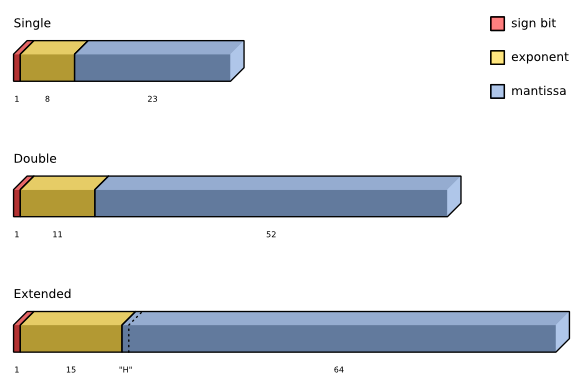
\includegraphics[scale = 0.45]{ieee-types.png}}
\end{frame}

\begin{frame}{Типы дробных чисел в C++}
    \begin{table}[H]
        \begin{center}
        \resizebox{\textwidth}{!}{%
                
                \begin{tabular}{|*{3}{c|}}
                \hline
                float & double & long double \\
                \hline
                32 бита (4 байта) & 64 бита (8 байт) & 80 бит (10 байт)\\
                
                \makecell{23 бит мантиссы \\ $\frac{log(2^{24})}{log(10)} \approx  7.22$} & 
                \makecell{52 бита мантиссы  \\ $\frac{log(2^{53})}{log(10)} \approx  15.95$} &
                \makecell{52 бита мантиссы \\ $\frac{log(2^{64})}{log(10)} \approx  19.27$
                }
                \\
                \makecell{Недостаточная\\точность\\ для задач геометрии!}
                &
                \makecell{Точность достаточная\\ для большинства задач} &
                \makecell{Нужна иногда\\ (когда нужно вывести\\ числа порядка $10^{9}$\\ с точностью $10^{-9}$)}
                \\
                \hline
                \end{tabular}
            }
            
        \end{center}
    \end{table} 
\end{frame}

\begin{frame}[fragile]{Сравнение дробных чисел}
    \begin{minted}{cpp}
    float a = 0.15 + 0.15
    float b = 0.1 + 0.2
    if(a == b) // can be false!
    if(a >= b) // can also be false!
    \end{minted}
    \pause
    \begin{minted}{cpp}
    const double EPS = 1e-6;
    ...
    bool equal(double a, double b)
    {
        return abs(a - b) < EPS;
    }
    \end{minted}
\end{frame}

\begin{frame}[fragile]{Дробные ноль и бесконечность}
    \begin{minted}{cpp}
    double x = 0.0, inf = 1/x; 
    cout << 1/x << " "  << -1/x; // inf -inf
    cout << inf * 0 << " " << -inf * 0; // -nan -nan
    \end{minted}
\end{frame}

\begin{frame}[fragile]{Ввод и вывод дробных чисел в C++}
    \begin{minted}{cpp}
    #include <iomanip>
    ...
    float fx = 1./25;
    double dx = 1./25;
    cout << setprecision(15);
    cout << fx; // 0.0399999991059303
    cout << dx; // 0.04

    cout << setprecision(20) << fixed;
    cout << fx; // 0.03999999910593032837
    cout << dx; // 0.04000000000000000083
    \end{minted}
\end{frame}

\begin{frame}[fragile]{Функции библиотеки <cmath>}
    \begin{minted}{cpp}
    cout << fixed << setprecision(15);
    double angle = 30;
    double angle_rad = 30 * M_PI/180;
    double back_to_angle = angle_rad * 180/M_PI;
    // 29.999999999999996
    \end{minted}
        \pause
        
    \begin{minted}{cpp}
    double x = 1e9;
    cout << x << endl; // 1000000000.0000000000
    cout << sqrt(x) * sqrt(x); // 999999999.9999998808
    if(1e4 == sqrt(1e4) * sqrt(1e4)) // true
    if(1e5 == sqrt(1e5) * sqrt(1e5)) // false
    \end{minted}
\end{frame}


\section{Векторы и операции с ними}
\begin{frame}{Понятие вектора}
    \textbf{Вектор} - 
     направленный отрезок прямой.\\
     Будем считать, что начало отрезка всегда лежит в точке $(0,0)$
     Вектор будет задаваться кординатами точки конца $(x, y)$.
    \center{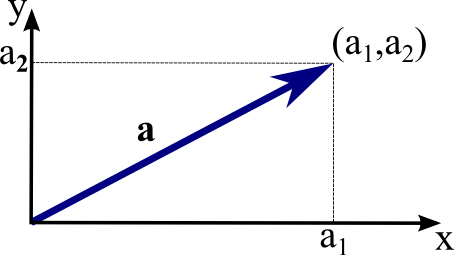
\includegraphics[scale = 1]{vector_2d_coordinates.png}}
\end{frame}
\begin{frame}{Свойства вектора}
    \textbf{Длина вектора}: $\left|\bf{a}\right| = \sqrt{a_{x}^{2} + a_{y}^{2}}$ \\
    \textbf{Сумма векторов}: $\bf{a} + \bf{b} = (a_{x} + b_{x}, a_{y} + b_{y})$\\
    \textbf{Разница векторов}: $\bf{a} - \bf{b} = (a_x - b_x, a_y - b_y)$
    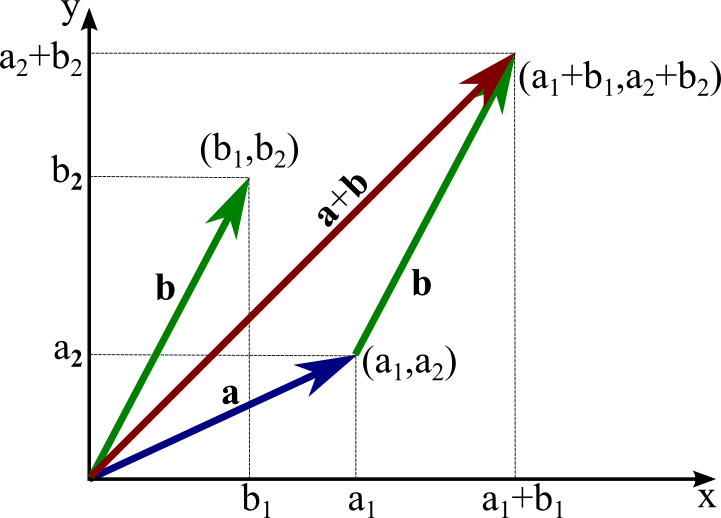
\includegraphics[scale = 0.6]{vector_2d_add.png}
\end{frame}

\begin{frame}{Скалярное произведение векторов}
    \begin{itemize}
        \item $\mathbf{a}\cdot\mathbf{b}
        =\left|\mathbf{a}\right|\left|\mathbf{b}\right|\cos\theta$
        \item $\mathbf{a}\cdot\mathbf{b}=a_x b_x + a_y b_y$
        \item Быстрый способ найти $\cos\theta = \frac{\mathbf{a}\cdot\mathbf{b}}{\left|\mathbf{a}\right|\left|\mathbf{b}\right|}$
        \item Быстрый способ найти информацию об угле(тупой,острый или прямой).Достаточно сравнить $\mathbf{a}\cdot\mathbf{b}$ и $0$.
    \end{itemize}
\end{frame}

\begin{frame}{Псевдоскалярное произведение}
    
    \begin{itemize}
        \item $\mathbf a \wedge \mathbf b=|\mathbf a|\cdot|\mathbf b|\sin\theta$
        \item $\theta = \angle(\mathbf{a}, \mathbf{b})$\\ угол вращения(против часовой стрелки) от $\mathbf a$ к
        $\mathbf b$
        \item $\mathbf{a} \wedge \mathbf{b} = \begin{vmatrix} a_x & a_y \\ b_x & b_y \end{vmatrix} = a_x \cdot b_y - b_x \cdot a_y$
        \pause
        \item Если сравнить $\mathbf{a} \wedge \mathbf{b}$ с нулём, то можно узнать расположение вектора \textbf{a} отнонсительно вектора \textbf{b}
        \item $\mathbf{a} \wedge \mathbf{b}$ равен площади параллелограмма, натянутого на эти вектора
        \item ** Угол между двумя векторами: $atan2(\mathbf{a}\cdot\mathbf{b}, \mathbf{a} \wedge \mathbf{b})$
    \end{itemize}
\end{frame}
\begin{frame}{Псевдоскалярное произведение}
    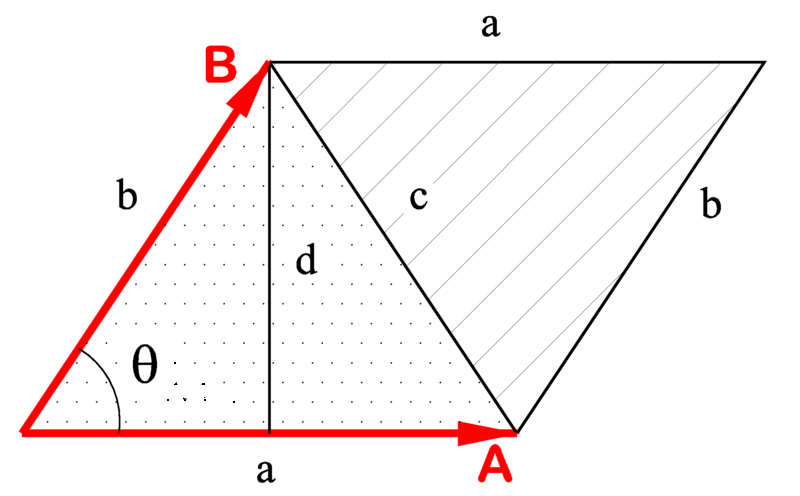
\includegraphics[scale = 0.35]{Magnitude_cross_product.png}
\end{frame}

\begin{frame}[fragile]{C++ Vector}
    \begin{minted}{cpp}
struct Vec {
	double x, y;

	Vec(double x, double y) :x(x), y(y) {}
	Vec() :x(0), y(0) {}

	inline double len_sqr() {
		return x*x + y*y;
	}
	inline double len() {
		return sqrt(x*x + y*y);
	}
	...
    	
    \end{minted}
\end{frame}

\begin{frame}[fragile]{C++ Vector}
    \begin{minted}{cpp}
    ...
    friend Vec operator*(const Vec & a, double k) {
        return Vec(a.x*k, a.y*k);
    }
    inline Vec normal() {
        if (len_sqr() == 0) return *this;
        double inv = 1 / len();
        return Vec(x*inv, y*inv);
    }
    inline Vec rot(double angle) {
        double sn = sin(angle);
        double cs = cos(angle);
        return Vec(x*cs - y*sn, x*sn + y*cs);
    }
    ...
    \end{minted}
\end{frame}

\begin{frame}[fragile]{C++ Vector}
    \begin{minted}{cpp}
    ...
    friend Vec operator+(const Vec & a, const Vec & b) {
        return Vec(a.x + b.x, a.y + b.y);
    }
    friend Vec operator-(const Vec & a, const Vec & b) {
        return Vec(a.x - b.x, a.y - b.y);
    }
    friend double operator*(const Vec & a, const Vec & b) {
        return a.x*b.x + a.y*b.y;
    }
    friend double operator^(const Vec & a, const Vec & b) {
        return a.x*b.y - a.y*b.x;
    }
}
    \end{minted}
\end{frame}
\section{Прямые и отрезки}
\begin{frame}{Пересечение двух прямых через уравнения прямых}
\begin{figure}
        \begin{tikzpicture}
        \draw[gray, thick] (-1,2) -- (2,-4);
        \draw[gray, thick] (-1,-1) -- (2,2);
        \filldraw[black] (0,0) circle (2pt) node[anchor=west] {Точка пересечения};
    \end{tikzpicture}
\end{figure}
\end{frame}

\begin{frame}{Пересечение двух прямых через уравнения прямых}
\begin{equation*}
 \begin{cases}
   A_1x + B_1y + C_1 = 0\\
   A_2x + B_2y + C_2 = 0
 \end{cases}
\end{equation*}
\begin{equation*}
 \begin{cases}
    x = - \frac{\begin{vmatrix}
C_1 & B_1\\
C_2 & B_2
\end{vmatrix}}{
\begin{vmatrix}
A_1 & B_1\\
A_2 & B_2
\end{vmatrix}
}
,y = - \frac{\begin{vmatrix}
A_1 & C_1\\
A_2 & C_2
\end{vmatrix}}{
\begin{vmatrix}
A_1 & B_1\\
A_2 & B_2
\end{vmatrix}
}\\
 \end{cases}
\end{equation*}
Эта система имеет решения, если прямые (1) и (2) не паралельные.
\end{frame}

\begin{frame}{Пересечение двух прямых через уравнения прямых}
    \begin{enumerate}
    \item Строим прямые по отрезкам
    \item Проверяем пересекаются ли прямые
    \item Находим точку пересечения прямых
    \item Проверяем принадлежит ли точка отрезкам
    \end{enumerate}
\end{frame}

\section{Многоугольники}
\begin{frame}{Площадь треугольника}
    Как найти площадь треугольника по кординатам?
    \pause
    $S(A,B,C)=\left|\frac{1}{2}(\overrightarrow{AB}\wedge \overrightarrow{AC})\right|$\\
    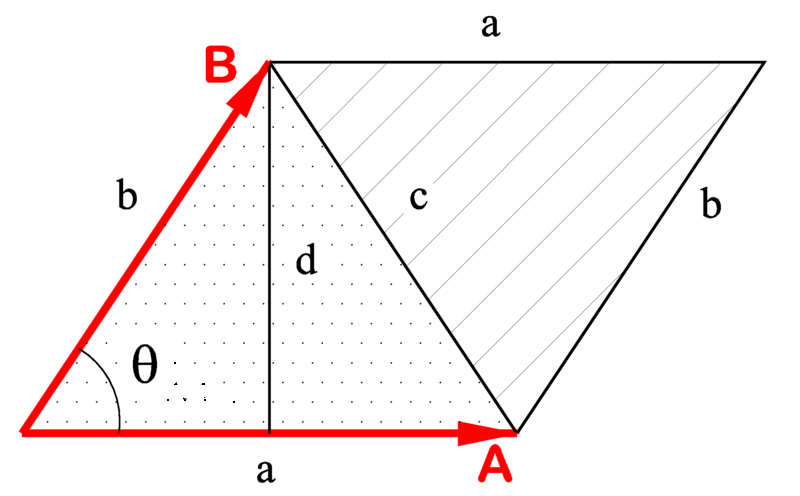
\includegraphics[scale = 0.2]{Magnitude_cross_product.png}
\end{frame}

\begin{frame}{Площадь многоугольника}
    \begin{figure}
            \begin{tikzpicture}
            \draw[gray, thick] (-3,-2) -- (-4,1) -- (-1,4) -- (4,3) -- (5,0) -- (2, -2) -- cycle;
            
            \pause
            
            \draw[black, thick] (-3,-2) -- (-1, 4);
            \draw[black, thick] (-3,-2) -- (4,3);
            \draw[black, thick] (-3,-2) -- (5, 0);
            
        \end{tikzpicture}
    \end{figure}
\end{frame}

\begin{frame}{Площадь многоугольника}
    \begin{figure}
            \begin{tikzpicture}
            \draw[black, thick] (-3,-2) -- (-1, 4);
            \draw[black, thick] (-3,-2) -- (4,3);
            \draw[black, thick] (-3,-2) -- (5, 0);
            
            \draw[gray, thick] (-3,-2) -- (-4,1) -- (-1,4) -- (4,3) -- (5,0) -- (2, -2) -- cycle;
            
            \filldraw[fill=green!20!white, draw=green!40!black] (-3,-2) -- (-4,1) -- (-1,4) -- cycle;
            \pause
            \filldraw[fill=green!20!white, draw=green!40!black] (-3,-2) -- (-1,4) -- (4,3) -- cycle;
            \pause
            
            \filldraw[fill=green!20!white, draw=green!40!black] (-3,-2) -- (4,3) -- (5,0) -- cycle;
            \pause
            
            \filldraw[fill=green!20!white, draw=green!40!black] (-3,-2) -- (5,0) -- (2, -2) -- cycle;
            
            \filldraw[black];
        \end{tikzpicture}
    \end{figure}
\end{frame}


\begin{frame}{Принадлежность точки многоугольнику}
    Как проверить принадлежит ли точка многоугольнику?
    
    \begin{figure}
            \begin{tikzpicture}
            \draw[gray, thick] (-3,-2) -- (-4,1) -- (-1,4) -- (4,3) -- (5,0) -- (2, -2) -- cycle;
            
            \filldraw[fill=green!20!white, draw=green!40!black] (2, 2) -- (-3,-2) -- (-4,1) -- cycle;
            \filldraw[fill=green!20!white, draw=green!40!black] (2, 2) -- (-4,1) -- (-1, 4) -- cycle;
            \filldraw[fill=green!20!white, draw=green!40!black] (2, 2) -- (-1, 4) -- (4,3) -- cycle;
            \filldraw[fill=green!20!white, draw=green!40!black] (2, 2)  -- (4,3) -- (5, 0) -- cycle;
            \filldraw[fill=green!20!white, draw=green!40!black] (2, 2)  -- (5, 0) -- (2, -2) -- cycle;
            \filldraw[fill=green!20!white, draw=green!40!black] (2, 2)  --  (2, -2) -- (-3,-2) -- cycle;
            
            \filldraw[black];
        \end{tikzpicture}
    \end{figure}
\end{frame}


\begin{frame}{Принадлежность точки многоугольнику}
    
    \begin{figure}
            \begin{tikzpicture}
            
            \filldraw[fill=green!20!white, draw=green!40!black] (6, 2)  -- (4,3) -- (5, 0) -- cycle;
            \filldraw[fill=green!20!white, draw=green!40!black] (6, 2) -- (-3,-2) -- (-4,1) -- cycle;
            \filldraw[fill=green!20!white, draw=green!40!black] (6, 2) -- (-4,1) -- (-1, 4) -- cycle;
            \filldraw[fill=green!20!white, draw=green!40!black] (6, 2) -- (-1, 4) -- (4,3) -- cycle;
            \filldraw[fill=green!20!white, draw=green!40!black] (6, 2)  -- (5, 0) -- (2, -2) -- cycle;
            \filldraw[fill=green!20!white, draw=green!40!black] (6, 2)  --  (2, -2) -- (-3,-2) -- cycle;
            
            \draw[gray, thick] (-3,-2) -- (-4,1) -- (-1,4) -- (4,3) -- (5,0) -- (2, -2) -- cycle;
            
            \filldraw[black];
        \end{tikzpicture}
    \end{figure}
\end{frame}

\begin{frame}{Целые точки}
    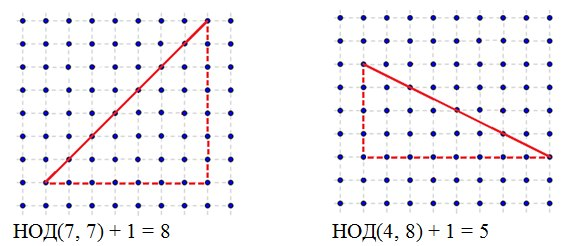
\includegraphics[scale = 0.7]{51c2fcc5fc47514d26a8ea8850cb1277.jpeg}
    
\end{frame}

\begin{frame}{Теорема Пика}
    $S = N_{inside} + \frac{N_{bound}}{2} - 1$\\
    \center{
    \includesvg[scale = 0.5]{Pick_theorem.svg}
    }
\end{frame}

\begin{frame}{Метод Монте-Карло}
    \center{
    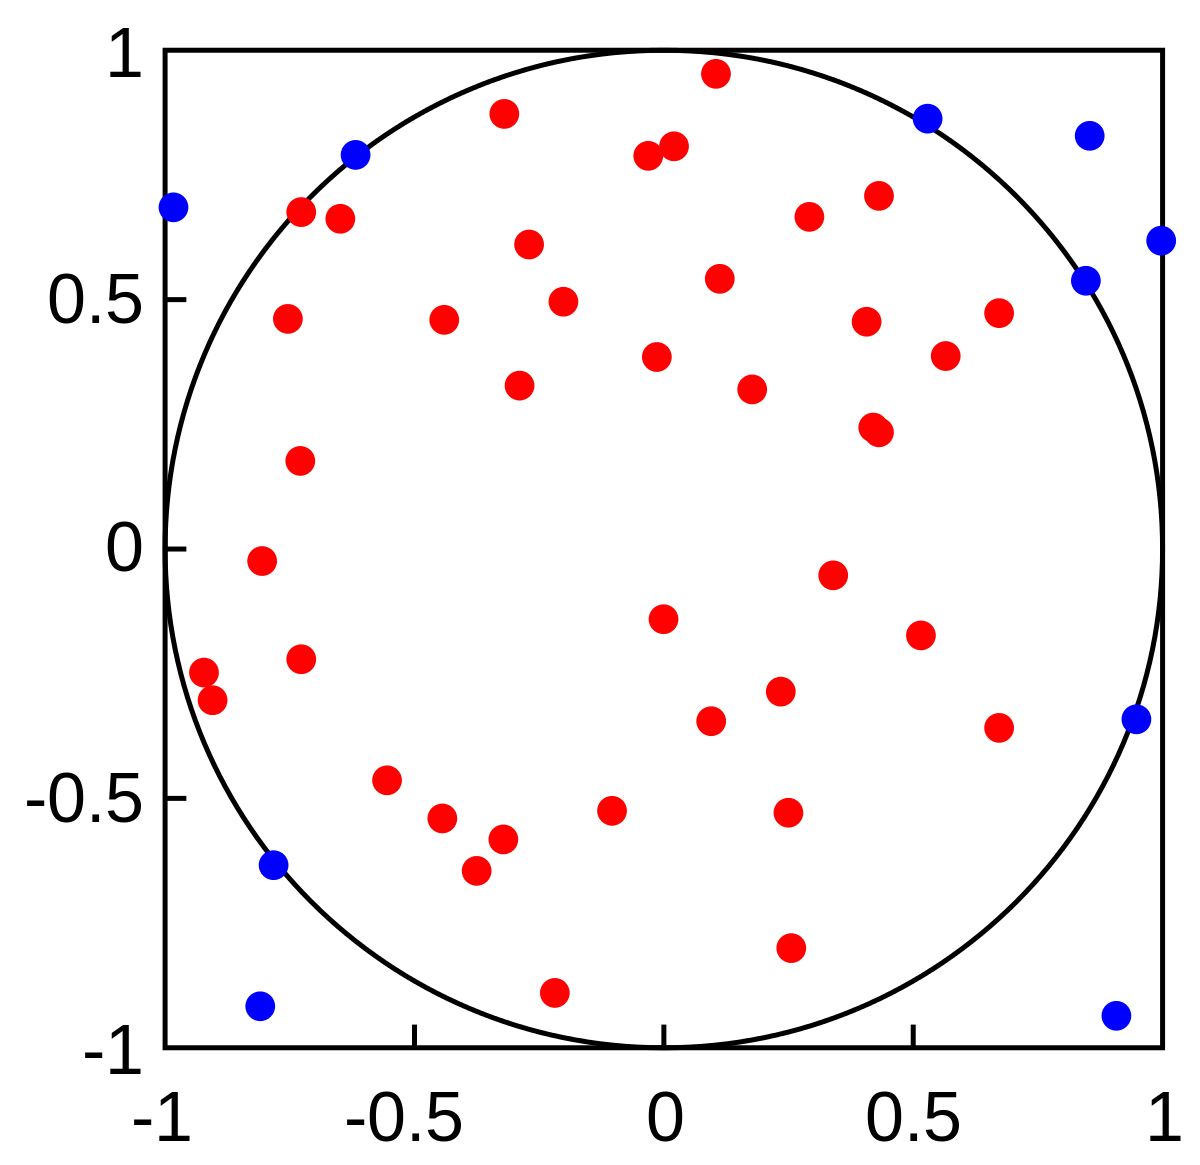
\includegraphics[scale = 0.18]{MonteCarloIntegrationCircle.png}
    }
\end{frame}

\section{Задачи}
\setlength{\parindent}{4em}
\begin{frame}{Задача №1}
    Четыре точки задают прямоугольник. Дано три точки, найти 4-ую\\
    \url{https://goo.gl/xE17Bm}
\end{frame}

\begin{frame}{Задача №2}
На лесной опушке растет дружная семейка грибов. Местоположение каждого гриба задается координатами X, Y, а шляпка гриба имеет радиус R.\par
Когда идет дождь, радиус шляпки каждого гриба непрерывно и равномерно увеличивается cо скоростью 1 сантиметр в минуту. \par
Когда дождь заканчивается (а он идет не более Т минут), шляпки прекращают расти. Если во время дождя шляпки двух грибов соприкоснулись, то они немедленно перестают расти, чтобы не навредить друг другу. \par
Грибы очень дружные, поэтому если перестают расти два гриба, то и все остальные тоже не растут.\par
Требуется посчитать, на сколько сантиметров увеличился радиус шляпки каждого гриба после завершения дождя.
\url{http://acmp.ru/index.asp?main=task&id_task=699}
\end{frame}


\begin{frame}{Задача №3}
У вас есть выпуклый многоугольник $P$, вершины которого расположены в n различных точках $p_1, p_2,\ldots, p_n$.\par Точка $p_i$ имеет координаты $(x_i, y_i)$ на плоскости. Точки перечислены в порядке обхода по часовой стрелке.\par
Задана точка $(x_0, y_0)$. Найти кратчайшее расстояние от точки $(x_0, y_0)$ до многоугольника $P$.
\par
\end{frame}

\begin{frame}{Задача №4}
На поле боя размещены $N$ имперских штурмовиков. Поле боя представляет собой плоскость с прямоугольной системой координат. Каждый штурмовик задан своими координатами $(x, y)$ на этой плоскости.\par
У Хана Соло есть новейшая двусторонняя лазерная пушка для сражения с этими штурмовиками. Она расположена в точке с координатами $(x_0, y_0)$. За один выстрел она способна поразить всех штурмовиков, находящихся на некоторой прямой, проходящей через точку $(x_0, y_0)$.\par
Требуется определить, за какое минимальное количество выстрелов Хан Соло сможет уничтожить всех штрумовиков.\par
\url{http://codeforces.com/problemset/problem/514/B}
\end{frame}

\begin{frame}{Задача №5}
У вас есть выпуклый многоугольник P, вершины которого расположены в n различных точках $p_1, p_2,\ldots, p_n$. Точка $p_i$ имеет координаты $(x_i, y_i)$ на плоскости. Точки перечислены в порядке обхода по часовой стрелке.\par
Вы можете выбрать вещественное число $D$ и передвинуть каждую из вершин многоугольника из начального положения в любую точку на расстоянии не больше $D$.\par
Найдите максимальное значение $D$ такое, что независимо от того, как вы передвинете вершины, многоугольник не пересечет сам себя и останется выпуклым.\par
\url{http://codeforces.com/problemset/problem/772/B}
\end{frame}


\begin{frame}{Задача №6}
На нескінченному полі знаходиться будівля, що має форму випуклого многокутника. До однієї з вершин цього многокутника на ланцюгу довжини L прив’язують вівцю. Знайти площу на якій зможе пастись вівця. Стіни будівлі є суцільними, вівця не може потрапити всередину будівлі. Вважається, що вівця може випасатись в будь-якій точці строго зовні будівлі, до якої може дійти.
\url{https://netoi.org.ua/index_ua.php?lng=ua&cid=1593}
\end{frame}

\begin{frame}{Задача №7*}
Дано $N$ разных точек $(x_1,y_1), (x_2, y_2), \cdots , (x_n, y_n)$. Гарантируется, что никакие три точки не лежат на одной прямой.\par
Выбрать из них 4 точки, так чтобы площадь четырехугольника построенного на этих точках была максимальна\par
\url{http://codeforces.com/problemset/problem/340/B}
\end{frame}

\begin{frame}{Задача №8*}
Недавно Роман, зайдя в класс, увидел, что на доске нарисовано $N$ точек. Разумеется, он сразу задумался, сколько существует троек из этих точек, которые являются вершинами равнобедренных треугольников.
\url{https://www.e-olymp.com/ru/problems/461}
\end{frame}


\begin{frame}{Задача №9*}
Задано поле N на M(из 0 и 1). На нем нарисована фигура(квадрат, круг или треугольник(произвольный)). Фигура состоит из единиц. Определить тип фигуры.

\url{http://acm.timus.ru/problem.aspx?num=1378&locale=ru}
\end{frame}


\begin{frame}{Вопросы!}
    \huge Вопросы?
\end{frame}

% All of the following is optional and typically not needed. 
\appendix
\section<presentation>*{\appendixname}
\subsection<presentation>*{}

\begin{frame}{Почитайте дома}
  Если много свободного времени:
  \url{https://www.e-olymp.com/ru/contests/8947}\\
  \url{https://www.e-olymp.com/ru/contests/9009}\\
  Более сложные алгоритмы и их реализация:
  \url{http://algolist.manual.ru/maths/geom/}\\
  Лекции по линейной алгебре[Eng]:\\
  \url{https://www.youtube.com/playlist?list=PLZHQObOWTQDPD3MizzM2xVFitgF8hE_ab}
\end{frame}

\end{document}